\documentclass[class=report, crop=false, 12pt,a4paper]{standalone}
\usepackage{enumitem}
\usepackage{gensymb}
\usepackage{pgfplots}
\usepackage{siunitx}
\usepackage{graphicx}
\usepackage{wrapfig}
\sisetup{detect-all}
\begin{document}
\textbf{Insert solid structure lab report here}
\section{}
\begin{tikzpicture}
  \begin{axis}[
      xmin=-0.5, xmax=2,
      ymin=-2, ymax=2,
      axis lines=center,
      axis on top=true,
      domain=0:1,
      ]
  
      \addplot [mark=none,draw=red,ultra thick] {2(1-1))};
  \end{axis}
\end{tikzpicture}
Energy 'well' asymmetric above $a_0$. Depth of the well is related to how 'stable' a material is in the solid state. This related to the melting point of the substance (and its chemical reactivity). Also as heat (energy) input into such a system, the minimum moves to the right hand side (as the well fills up). This predicts that $a_0$ increases as heat is input i.e. materials expands on heating - expansion coefficient.
\section{Solidification of crystalline materials}
Regular solid (crystalline) that forms at freezing point starts out via formation of nuclei (small 'areas' (embryos) of crystalline material). These are nominally 200-300 atoms in diameter. They come about randomly, via collisions; this process is called nucleation. Once a nucleus of a given critical size has been created, crystals become stable at $R_{crit}$ and more atoms join, leading to the crystal growing. Anything smaller than $R_{crit}$, the crystal will remelt (because we are at the melting point as well as the freezing point). Because nuclei become stable, the heat (energy) they lose, needs to be removed, else solidification (into the surroundings) will stop (latent heat of solidification). This process is isothermal at the melting point and can be monitored using a cooling curve. Nucleating, being random, can occur anywhere and everywhere. This results in many crystals being formed and a polycrystalline solid being formed.
\subsection{Practical casting}
\begin{figure}[h!]
  \begin{minipage}[b]{0.3\textwidth}
    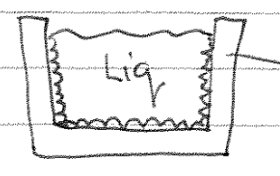
\includegraphics[width = \linewidth]{../img/practicalcasting1}
  \end{minipage}
  \hfill
  \begin{minipage}[b]{0.3\textwidth}
    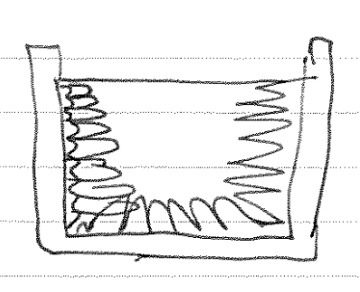
\includegraphics[width = \linewidth]{../img/practicalcasting2}
  \end{minipage}
  \hfill
  \begin{minipage}[b]{0.3\textwidth}
    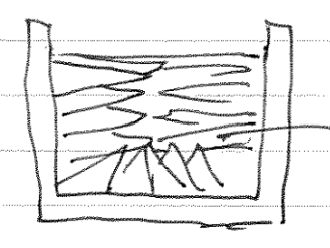
\includegraphics[width = \linewidth]{../img/practicalcasting3}
  \end{minipage}  
\end{figure}
Many nuclei but on walls of the mould. Many crystals with no orientation relationship between each other. Usually because this where the latent is being removed. Long thin "columna" crystals (grains). (WRT the crystal structure) and orientation. Hence misorientated crystals cannot join perfecttly. Polycrystalline solid grain structure aka microstructure um-mm in dimension. Strongly influences properties and can easily be altered via manufacturing processing. e.g. columna grains - typical of an 'open' casting are not ideal - better mechanical properties if grains are polygonal and approximately equal sized in 3 orthogonal directions: equiaxed crystals. Can be acheived (e.g. via rapid cooling)

\begin{figure}[h!]
  \centering
  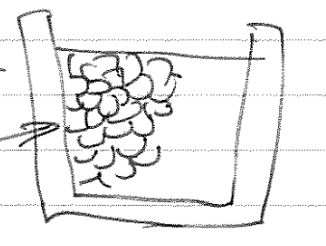
\includegraphics[width = 0.4\textwidth]{../img/equiaxed}
\end{figure}
When grains eventually touch they cant join perfectly - so they create an area of 'disorder' - i.e. high energy (thermodynamically) - not fully crystalline. This is the grain boundary. due to higher free energy. GB's are more likely to host chemical reactions or processes that decrease free energy. e.g. oxidation/corrosion. also significant in determining mechanical properties. during cooling if a material is very pure, it is possible to avoid nucleation and hence cool to below freezing point. This is called undercooling. n.b. extreme undercooling - called supercooling and results in no crystalline - re amorphous solids (supercooled, high viscosity liquids)
\begin{figure}[h!]
  \centering
  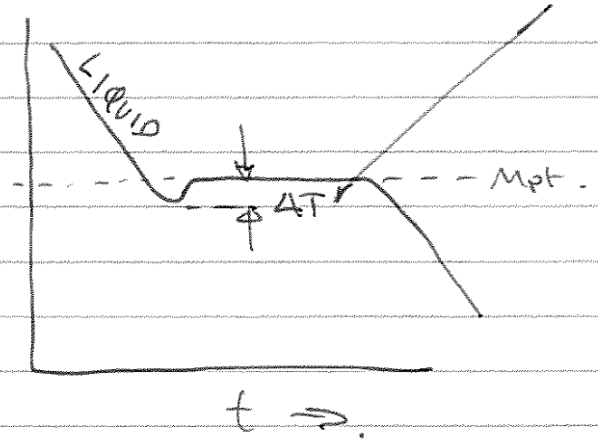
\includegraphics[width = 0.4\textwidth]{../img/supercooling}
\end{figure}
Once nucleation begins, the crystallisation process wil rapidly occur. Latent heat emerges and temperature rise to upt. undercooling can be generated by reapid cooling of a mould. more common in materials that find it difficult to crystallize e.g. long chain thermopolymers and si02 ceramics. undercooling therefore occurs more easily in complex crystal structures structures - in a metal delta T is almost impossible to observe. Possible to see in ultra pure metals and/or if cast into a very clean mould. why? delta T is related to the time it takes to create stable nuclei - i.e. reach $R_{crit}$ 

$R_{crit}$ is a radius - achievable either by creating a sphere of atoms or a hemisphere of atoms.
\begin{figure}[h!]
  \begin{minipage}[b]{0.45\textwidth}
    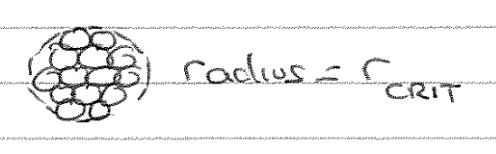
\includegraphics[width = \linewidth]{../img/rcritfull}
  \end{minipage}
  \hfill
  \begin{minipage}[b]{0.45\textwidth}
    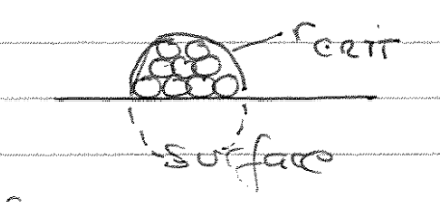
\includegraphics[width = \linewidth]{../img/rcrithalf}
  \end{minipage} 
\end{figure}
Thus, if a surface is available it can reduce the requirement for the no of atoms to create $R_{crit}$ (was a random process - so more chance of happening). i.e. surfaces help nucleation and act as sites for nucleation. There are two types of nucleation that we can define: self nucleation (homogeneous nucleation) and heterogeneous (nucleation on something). Nucleation type affects microstructure. 
\begin{figure}[h!]
  \begin{minipage}[b]{0.45\textwidth}
    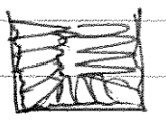
\includegraphics[width = \linewidth]{../img/heteronucleation}
    \caption{Heterogeneous nucleation X1}
  \end{minipage}
  \hfill
  \begin{minipage}[b]{0.45\textwidth}
    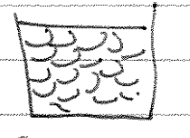
\includegraphics[width = \linewidth]{../img/homonucleation}
    \caption{Homogeneous nucleation (or hetero if impure) X1A}
  \end{minipage} 
\end{figure}
Commercially done by adding innoculants e.g. Ti02 Si02 powder. Also known as seeding. 

In many crystalline solids, the process of solidification goes through a dendritic stage. dendrite - from greek for tree - dendra - 3D crystal
\begin{figure}[h!]
  \begin{minipage}[b]{0.45\textwidth}
    \centering
    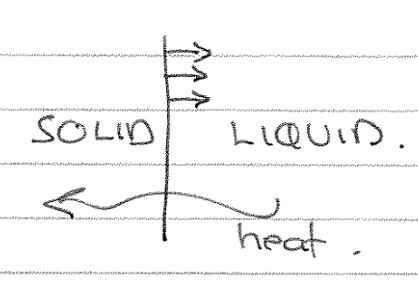
\includegraphics[width = 0.75\linewidth]{../img/dendriticgrowth4}
  \end{minipage}
  \hfill
  \begin{minipage}[b]{0.45\textwidth}
    \centering
    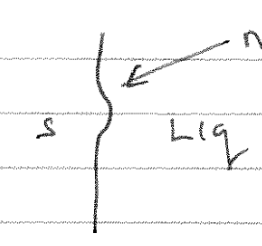
\includegraphics[width = 0.75\linewidth]{../img/dendriticgrowth3}
  \end{minipage} 
\end{figure}
Dendrites emerge from nominally stable S-L growth fronts and would normally melt back - but under certain circumstances any protruberance becomes stable
\begin{figure}
  \centering
  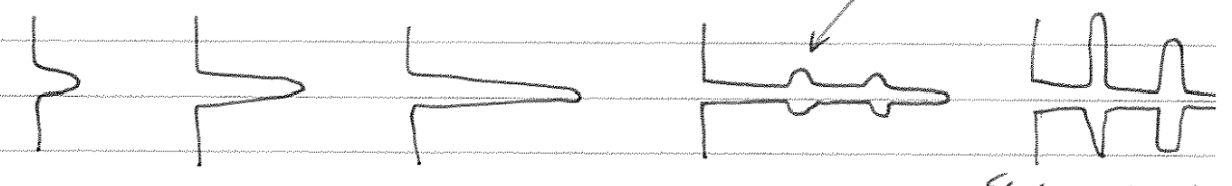
\includegraphics[width = \textwidth]{../img/dendriticgrowth2}
\end{figure}
e.g. see constitutional supercooling. more likely in impure substances
\begin{figure}[h!]
  \centering
  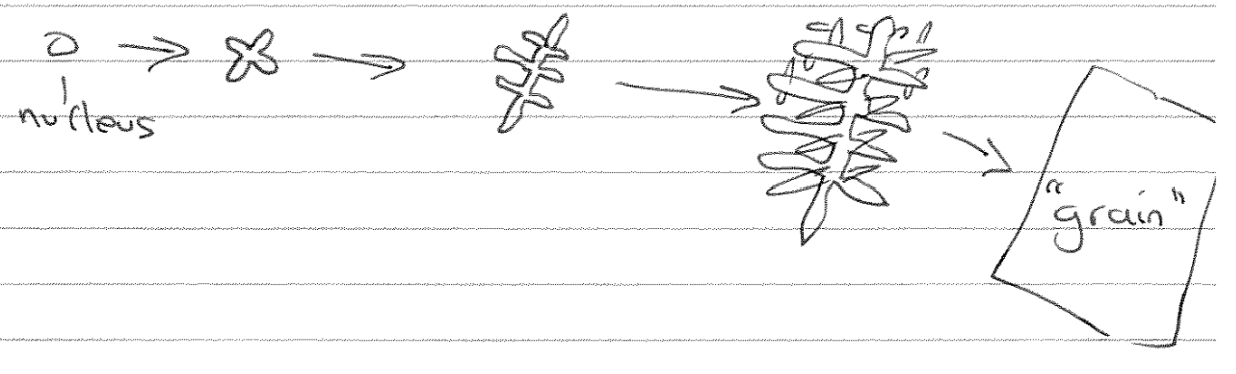
\includegraphics[width = \textwidth]{../img/dendriticgrowth}
\end{figure}
normally a growing dendrite will fill space gradually and become a single crystal and in disappear. 

Two occasions when dendrites appear in the microstructure: coring - variation in the composition of a dendrite as it grows revealing the stages of dendritic growth e.g. as colour changes. gradual change in composition - microsegregation. every grain will be cored, can compromise corrosion resistance and mechanical properties. or if the space in between the dendrite arms are filled with another substance (phase see X6 and X7). 

in casting technology, coring is regarded as a defect but there are others, principally porosity - holes in the microstructure. they can seriously degreade/affect mechanical properties. act as stress concentrators. 
\end{document}